\section{Proposed Method}
\label{sec:method}
% Intuition - why should it be better than the state of the art?
% Description of its algorithms
In this project, we explore three neural network models---single-layer
neural network (Logistic Regression), Multi-layer Logistic Regression
(MLP), Convolutional Neural Network (LeNet).
Figure~\ref{fig:networks} shows two neural network models: MLP and LeNet.
\begin{figure}[!htbp]
\centering
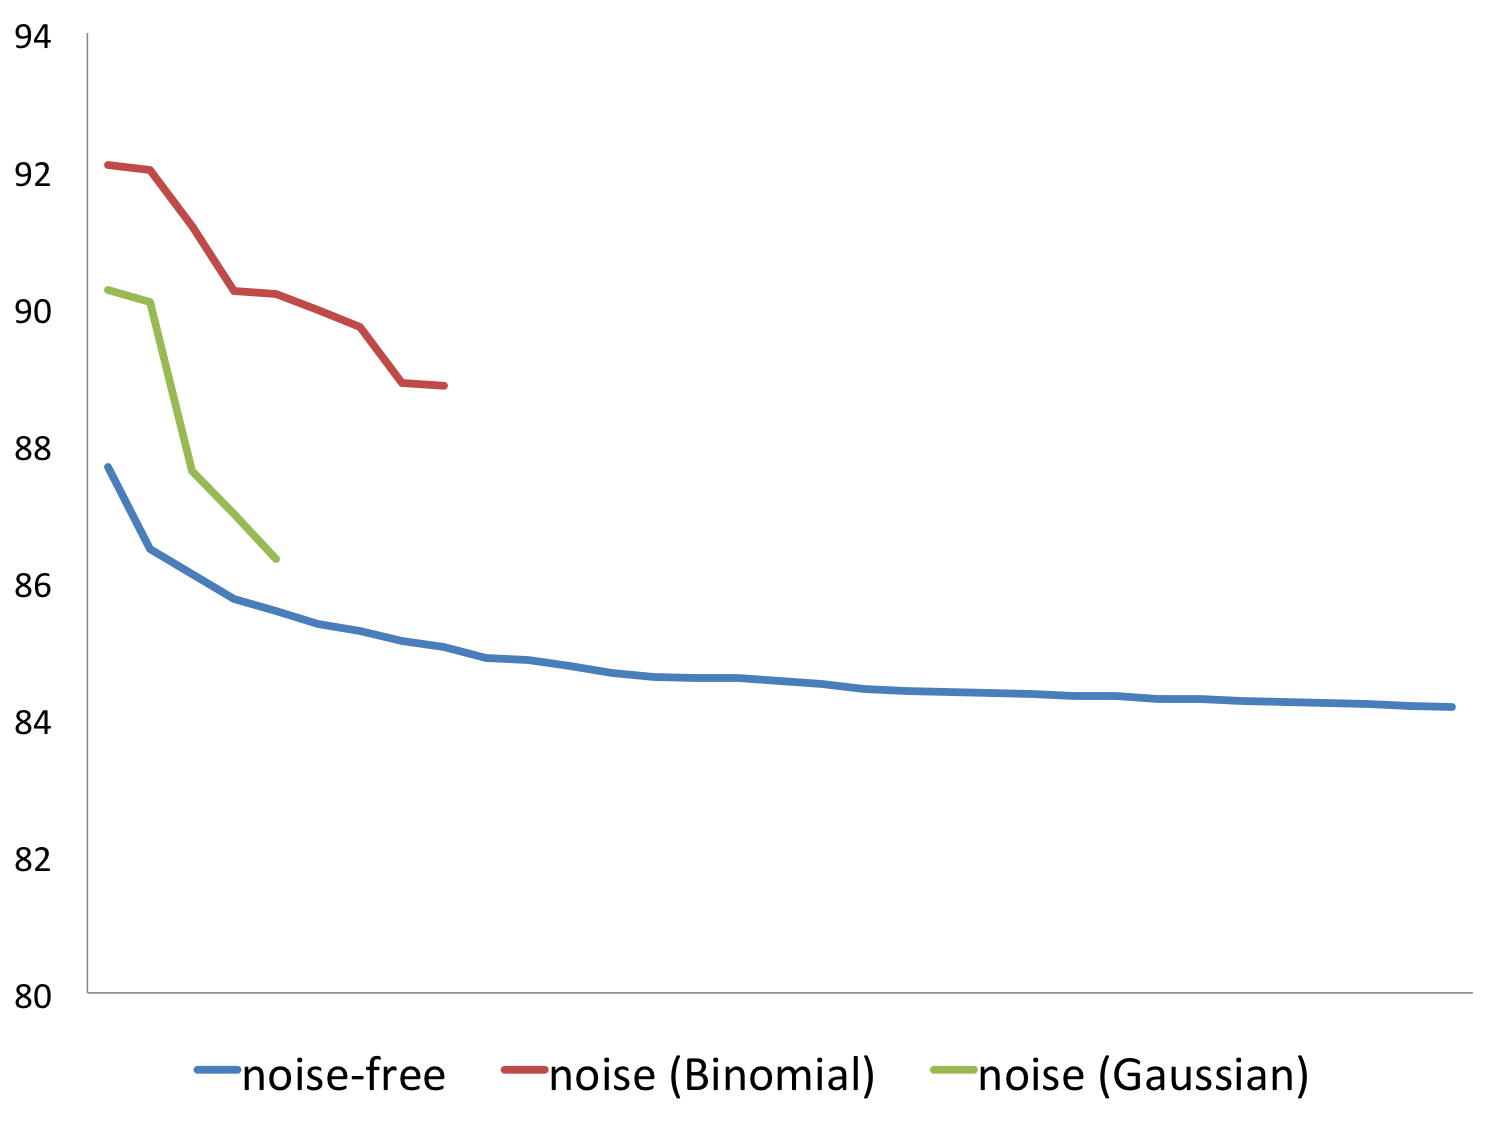
\includegraphics[width=295pt]{f-figs/networks}
\caption{Neural Network Models}
\label{fig:networks}
\end{figure}

\subsection{Adding Noise into Logistic Regression}
We first intorduce noise into gradient descent component
of Logistic Regression.
To be more specific, in a noise-free Logistic Regression model, weights
are updated in the following way:
\[
W_{new} = W_{old} - \lr \nabla_{W_{old}} \cost(W)
\]
In a noise-added Logistic Regression model, weights are updated as:
\[
W_{new}=W_{old}-\lr \left(\mask \cdot \nabla_{W_{old}}\cost(W) \right)
\]
or
\[
W_{new} = W_{old} - \mask_{Gau} \cdot \nabla_{W_{old}} \cost(W)
\]
where learning rate is a scalar and mask is a vector that has the same dimension as $W_t$.
We generate $mask$ as a random vector from Binomial distribution
$Bin(1,0.5)$, Gaussian distribution $\mathcal{N}(\lr, 2 \cdot \lr)$,
Rayleigh Distribution or Gamma Distribution $Gamma(1)$.

\subsection{Adding Noise into Multi-layer Logistic Regression}
Secondly, we introduce noise into weights between layers.
In our Multi-layer Logistic Regression model, there are three layers:
input layer, hidden layer and output layer. Each layer consists of
neurons. Neurons in different layers are connected by weights.

During a noise-free training process of the model, weights between layers
are transmitted and updated without any loss of information or variances.
However, during a noise-added training process, weights between layers are
are subject to some variation.
To be more specific, let $W_{input}$ be the matrix of weights between
input layer and hidden layer, $W_{output}$ be the matrix of weights
between hidden layer and output layer. In a noise-added training procoss,
we add combination of the following steps:
\begin{align*}
W_{input} & = W_{input} \cdot mask \\
W_{output} & = W_{output} \cdot mask \\
W_{input} & = W_{input} + mask
\end{align*}
where mask is a matrix of the same dimension as $W_{input}$ or $W_{output}$.
We generate mask as a random matrix from Binomial Distribution
$Bin(1,0.99)$ or Gaussian Distribution $\mathcal{N}(0, 0.01)$.

\subsection{Adding Noise into Convolutionary Neural Network}
Last, we introduce noise into feature mapping component of
the model. The difference between Convolutionary Neural Network and
Multi-layer Logistic Regression is that it has a feature mapping process
before MLP. Feature mapping is the process where a small window moves along
the image to extract local features. In other words, the window, acting as
a function, will compute a linear combination of the underlying pixels.
In a noise-added feature mapping process, the extracted feature is subject
to some variation.
